\documentclass[12pt]{article}
	
\usepackage[margin=1in]{geometry}
\usepackage{amsmath, amssymb}
\usepackage{fancyhdr}
\usepackage{graphicx}
\graphicspath{{imagenes/}{./}}
\usepackage{cancel}
\usepackage[spanish, es-tabla]{babel}
\usepackage{hyperref}
\usepackage{listings}
\usepackage{xcolor}
\usepackage{booktabs}

% Paleta de colores para codigo
\definecolor{codegreen}{rgb}{0.13,0.55,0.13}
\definecolor{codegray}{rgb}{0.5,0.5,0.5}
\definecolor{codepurple}{rgb}{0.58,0,0.82}
\definecolor{backcolour}{rgb}{0.97,0.98,0.99}

\lstdefinestyle{customcode}{
    backgroundcolor=\color{backcolour},   
    commentstyle=\color{codegreen}\itshape,
    keywordstyle=\color{blue}\bfseries,
    numberstyle=\tiny\color{codegray},
    stringstyle=\color{codepurple},
    basicstyle=\ttfamily\footnotesize,
    breakatwhitespace=false,         
    breaklines=true,                 
    captionpos=b,                    
    keepspaces=true,                 
    numbers=left,                    
    numbersep=6pt,                  
    showspaces=false,                
    showstringspaces=false,
    showtabs=false,                  
    tabsize=4,
    frame=single,
    rulecolor=\color{black!20}
}

\lstset{style=customcode}

\hypersetup{
    colorlinks=true,
    linkcolor=blue!80!black,
    urlcolor=blue!80!black,
    citecolor=blue!80!black
}

%%%%%%%%%%%%%%%%%%%%%%
% Configuracion de encabezado y pie de pagina
\pagestyle{fancy}
\fancyhead[LO,L]{\small Estructura de Datos}
\fancyhead[CO,C]{\small FINESI - UNA PUNO}
\fancyhead[RO,R]{\small 2026}
\fancyfoot[LO,L]{\small Prof. Fred Torres Cruz}
\fancyfoot[CO,C]{\small Página \thepage}
\fancyfoot[RO,R]{\small Henry Mamani Gutierrez}
\renewcommand{\headrulewidth}{0.4pt}
\renewcommand{\footrulewidth}{0.4pt}
%%%%%%%%%%%%%%%%%%%%%%

\begin{document}

% ENCABEZADO INSTITUCIONAL CON LOGOS
\begin{minipage}{0.18\textwidth}
    
\includegraphics[width=2.4cm]{logo-una-puno.png}
\end{minipage}
\hfill
\begin{minipage}{0.60\textwidth}
    \centering
    \textbf{\large UNIVERSIDAD NACIONAL DEL ALTIPLANO DE PUNO}\\[1.5mm]
    \textbf{\small FACULTAD DE INGENIERÍA ESTADÍSTICA E INFORMÁTICA}\\[1mm]
    \textbf{\footnotesize ESCUELA PROFESIONAL DE INGENIERÍA ESTADÍSTICA E INFORMÁTICA}
\end{minipage}
\hfill
\begin{minipage}{0.18\textwidth}
    \centering
    
\includegraphics[width=2.4cm]{logofinesi.png}
\end{minipage}

\vspace{4mm}
\hrule height 1pt
\vspace{4mm}

\noindent \textbf{Curso:} Estructura de Datos (2026) \\
\textbf{Docente:} Prof. Fred Torres Cruz \\
\textbf{Autor / Estudiante:} Henry Antonio Mamani Gutierrez \\
\textbf{Correo Institucional:} \texttt{henrymamani@est.unap.edu.pe} \\
\textbf{Repositorio General (GitHub):} \url{https://github.com/henrymamani-alt/henry-ejercicios}

\vspace{4mm}
\noindent\textbf{\Large Trabajo Encargado - N° 001: Estructuras Básicas}\\
\noindent\rule{\textwidth}{0.5pt}

\section*{Presentación del Trabajo}
El presente trabajo encargado contiene la solución detallada de los 15 ejercicios del \textbf{Capítulo I: Estructuras Básicas}. Cada ejercicio cuenta con:
\begin{enumerate}
    \item \textbf{Enunciado oficial} asignado en la guía de práctica.
    \item \textbf{Análisis y explicación algorítmica} de la solución.
    \item \textbf{Código fuente completo} (en C o C++ según lo requerido).
    \item \textbf{Enlace directo} al código fuente en el repositorio GitHub.
    \item \textbf{Evidencia de ejecución} mediante captura gráfica de la consola de comandos.
\end{enumerate}

\newpage

% ========================================================
% EJERCICIO 1
% ========================================================
\section*{Ejercicio 1: Cálculo de Costo de Procesamiento por Analista}
\addcontentsline{toc}{section}{Ejercicio 1: Cálculo de Costo de Procesamiento por Analista}

\noindent\textbf{Enunciado:}\\
\textit{Desarrolle un programa en C que registre las horas dedicadas por un analista al procesamiento de un conjunto de datos y el costo por hora. Calcule el costo total del procesamiento y muestre un resumen con las horas trabajadas, tarifa aplicada y costo final.}

\subsection*{Análisis del Algoritmo}
Se solicitan dos variables numéricas en coma flotante (\texttt{float}): \texttt{horas\_trabajadas} y \texttt{costo\_por\_hora}. La tarifa final es el producto directo de ambos valores:
\[ \text{Costo Total} = \text{Horas Trabajadas} \times \text{Tarifa por Hora} \]
Se valida que ambas entradas sean valores no negativos.

\subsection*{Código Fuente en C (\texttt{ejercicio1.c})}
\noindent\textbf{Enlace al Repositorio:} \url{https://github.com/henrymamani-alt/henry-ejercicios/blob/main/Tarea_1_Estructuras_Basicas/codigo/ejercicio1.c}

\begin{lstlisting}[language=C]
#include <stdio.h>

int main() {
    float horas_trabajadas;
    float costo_por_hora;
    float costo_total;

    printf("=====================================================\n");
    printf("   CALCULO DE COSTOS DE PROCESAMIENTO DE DATOS      \n");
    printf("=====================================================\n");

    printf("Ingrese las horas dedicadas por el analista: ");
    if (scanf("%f", &horas_trabajadas) != 1 || horas_trabajadas < 0) {
        printf("Error: Entrada invalida para horas trabajadas.\n");
        return 1;
    }

    printf("Ingrese la tarifa (costo por hora en S/.): ");
    if (scanf("%f", &costo_por_hora) != 1 || costo_por_hora < 0) {
        printf("Error: Entrada invalida para costo por hora.\n");
        return 1;
    }

    costo_total = horas_trabajadas * costo_por_hora;

    printf("\n---------------- RESUMEN DE PROCESAMIENTO -----------\n");
    printf(" Horas trabajadas : %.2f hrs\n", horas_trabajadas);
    printf(" Tarifa aplicada  : S/. %.2f por hora\n", costo_por_hora);
    printf(" Costo total final: S/. %.2f\n", costo_total);
    printf("-----------------------------------------------------\n");

    return 0;
}
\end{lstlisting}

\subsection*{Evidencia de Ejecución}
\begin{center}
    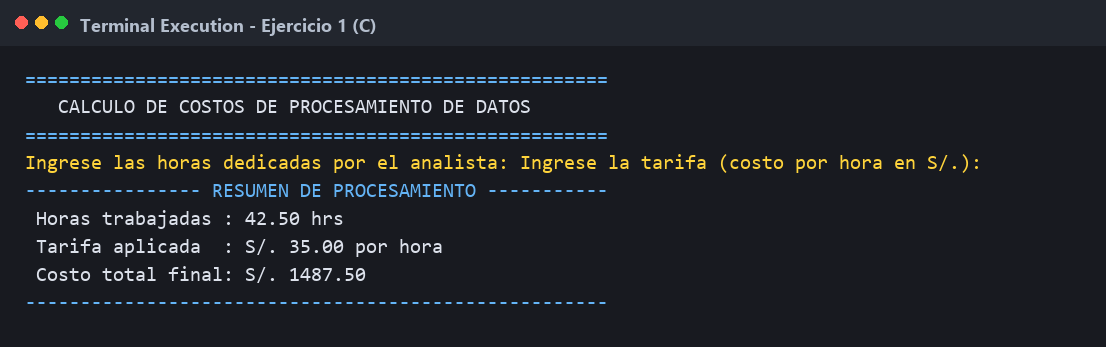
\includegraphics[width=0.92\textwidth]{captura_ejercicio1.png}
\end{center}

\vspace{5mm}
\hrule
\newpage

% ========================================================
% EJERCICIO 2
% ========================================================
\section*{Ejercicio 2: Registro de Observación de Datos y Tipos de Datos}
\addcontentsline{toc}{section}{Ejercicio 2: Registro de Observación de Datos y Tipos de Datos}

\noindent\textbf{Enunciado:}\\
\textit{Desarrolle un programa en C que registre información básica de una observación de un conjunto de datos: identificador, edad, valor promedio de una variable, categoría representada por una letra y estado de validez del registro. Utilice tipos de datos apropiados y muestre la información almacenada.}

\subsection*{Análisis del Algoritmo}
Se seleccionan tipos de datos exactos:
\begin{itemize}
    \item \texttt{int}: Identificador numérico (\texttt{id}) y la \texttt{edad}.
    \item \texttt{double}: Valor promedio de variable cuantitativa continua con doble precisión.
    \item \texttt{char}: Letra representativa de la categoría cualitativa.
    \item \texttt{bool}: Indicador lógico binario de validez (\texttt{stdbool.h}).
\end{itemize}

\subsection*{Código Fuente en C (\texttt{ejercicio2.c})}
\noindent\textbf{Enlace al Repositorio:} \url{https://github.com/henrymamani-alt/henry-ejercicios/blob/main/Tarea_1_Estructuras_Basicas/codigo/ejercicio2.c}

\begin{lstlisting}[language=C]
#include <stdio.h>
#include <stdbool.h>

int main() {
    int id;                      // Identificador unico (entero)
    int edad;                    // Edad de la observacion (entero)
    double valor_promedio;       // Valor promedio de variable (double)
    char categoria;              // Categoria representada por una letra
    bool es_valido;              // Estado de validez del registro
    int entrada_validez;

    printf("=====================================================\n");
    printf("        REGISTRO DE OBSERVACION DE DATOS             \n");
    printf("=====================================================\n");

    printf("Ingrese ID del registro (ej. 101): ");
    scanf("%d", &id);

    printf("Ingrese la edad del individuo: ");
    scanf("%d", &edad);

    printf("Ingrese el valor promedio de la variable (ej. 84.75): ");
    scanf("%lf", &valor_promedio);

    printf("Ingrese la categoria (letra A, B, C, etc.): ");
    scanf(" %c", &categoria);

    printf("Estado de validez (1 = Valido, 0 = Invalido): ");
    scanf("%d", &entrada_validez);
    es_valido = (entrada_validez != 0);

    printf("\n================ RESUMEN DE OBSERVACION =============\n");
    printf(" [1] Identificador (int)        : %d\n", id);
    printf(" [2] Edad (int)                 : %d anios\n", edad);
    printf(" [3] Valor Promedio (double)    : %.4f\n", valor_promedio);
    printf(" [4] Categoria (char)           : %c\n", categoria);
    printf(" [5] Estado de Validez (bool)   : %s\n", es_valido ? "VALIDO (true)" : "INVALIDO (false)");
    printf("=====================================================\n");

    return 0;
}
\end{lstlisting}

\subsection*{Evidencia de Ejecución}
\begin{center}
    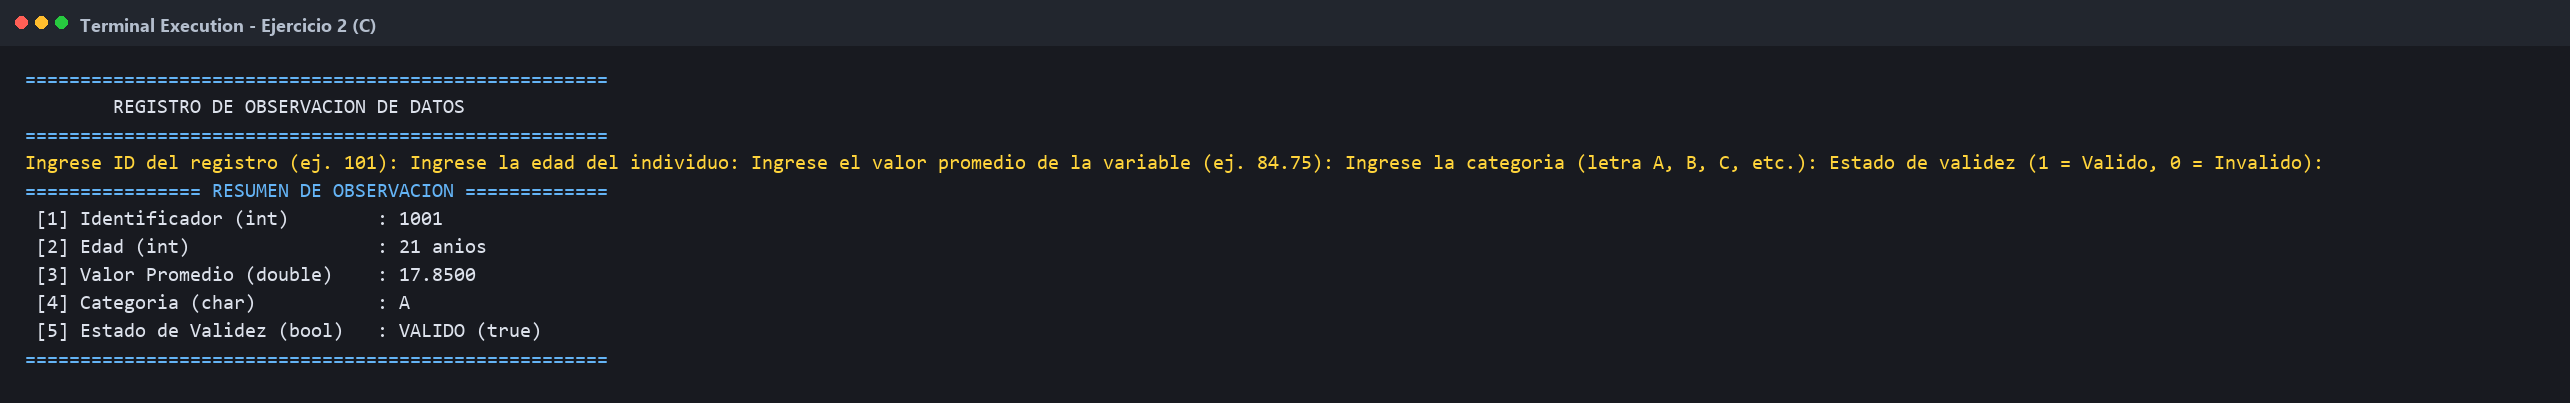
\includegraphics[width=0.92\textwidth]{captura_ejercicio2.png}
\end{center}

\vspace{5mm}
\hrule
\newpage

% ========================================================
% EJERCICIO 3
% ========================================================
\section*{Ejercicio 3: Conversión Explícita (Casting) y Pérdida Decimal}
\addcontentsline{toc}{section}{Ejercicio 3: Conversión Explícita (Casting) y Pérdida Decimal}

\noindent\textbf{Enunciado:}\\
\textit{Desarrolle un programa en C que solicite una medición decimal obtenida por un sensor, por ejemplo 18.9, la convierta explícitamente a un valor entero y muestre ambos resultados. Indique mediante la salida del programa cuánto valor decimal se pierde durante la conversión.}

\subsection*{Análisis del Algoritmo}
Se demuestra el operador de moldeo o casting \texttt{(int)medicion\_decimal}. Este operador trunca la parte fraccionaria. La pérdida resultante se cuantifica evaluando la diferencia entre el flotante original y su proyección entera convertida.

\subsection*{Código Fuente en C (\texttt{ejercicio3.c})}
\noindent\textbf{Enlace al Repositorio:} \url{https://github.com/henrymamani-alt/henry-ejercicios/blob/main/Tarea_1_Estructuras_Basicas/codigo/ejercicio3.c}

\begin{lstlisting}[language=C]
#include <stdio.h>

int main() {
    double medicion_decimal;
    int medicion_entera;
    double valor_perdido;

    printf("=====================================================\n");
    printf("    CONVERSION EXPLICITA (CASTING) DE SENSOR         \n");
    printf("=====================================================\n");

    printf("Ingrese la medicion decimal del sensor (ej. 18.9): ");
    if (scanf("%lf", &medicion_decimal) != 1) {
        printf("Error: Entrada invalida.\n");
        return 1;
    }

    // Conversion explicita (casting) a entero
    medicion_entera = (int)medicion_decimal;

    // Calculo del valor decimal que se pierde
    valor_perdido = medicion_decimal - (double)medicion_entera;

    printf("\n---------------- RESULTADOS DE CONVERSION -----------\n");
    printf(" Valor original (decimal) : %.4f\n", medicion_decimal);
    printf(" Valor convertido (entero): %d\n", medicion_entera);
    printf(" Valor decimal perdido    : %.4f\n", valor_perdido);
    printf(" Porcentaje de perdida    : %.2f%%\n", (valor_perdido / medicion_decimal) * 100.0);
    printf("-----------------------------------------------------\n");

    return 0;
}
\end{lstlisting}

\subsection*{Evidencia de Ejecución}
\begin{center}
    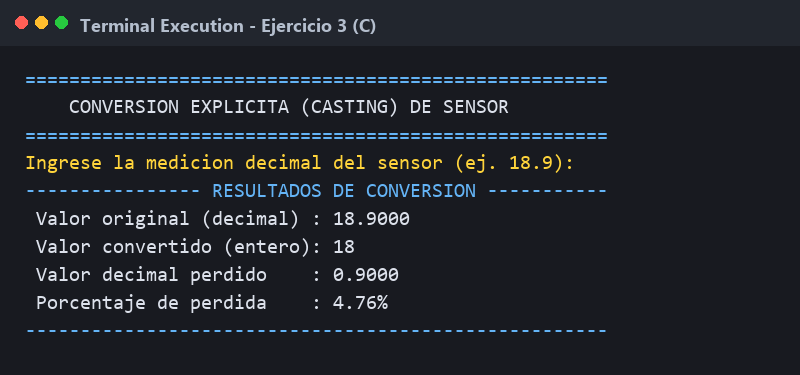
\includegraphics[width=0.92\textwidth]{captura_ejercicio3.png}
\end{center}

\vspace{5mm}
\hrule
\newpage

% ========================================================
% EJERCICIO 4
% ========================================================
\section*{Ejercicio 4: Operaciones Aritméticas entre Registros Procesados}
\addcontentsline{toc}{section}{Ejercicio 4: Operaciones Aritméticas entre Registros Procesados}

\noindent\textbf{Enunciado:}\\
\textit{Desarrolle un programa en C que solicite dos valores enteros correspondientes al número de registros procesados por dos algoritmos. Calcule suma, diferencia, producto, división entera y residuo, y muestre los resultados de manera organizada.}

\subsection*{Análisis del Algoritmo}
Se solicitan dos cantidades enteras y se procesan las cinco operaciones aritméticas básicas de C (\texttt{+}, \texttt{-}, \texttt{*}, \texttt{/}, \texttt{\%}). Se implementa control defensivo en la división y el residuo para evitar excepciones por división entre cero.

\subsection*{Código Fuente en C (\texttt{ejercicio4.c})}
\noindent\textbf{Enlace al Repositorio:} \url{https://github.com/henrymamani-alt/henry-ejercicios/blob/main/Tarea_1_Estructuras_Basicas/codigo/ejercicio4.c}

\begin{lstlisting}[language=C]
#include <stdio.h>

int main() {
    int reg_algoritmo1;
    int reg_algoritmo2;

    printf("=====================================================\n");
    printf("   COMPARATIVA Y ARITMETICA DE REGISTROS (ALGORITMOS)\n");
    printf("=====================================================\n");

    printf("Ingrese registros procesados por Algoritmo 1: ");
    scanf("%d", &reg_algoritmo1);

    printf("Ingrese registros procesados por Algoritmo 2: ");
    scanf("%d", &reg_algoritmo2);

    int suma = reg_algoritmo1 + reg_algoritmo2;
    int diferencia = reg_algoritmo1 - reg_algoritmo2;
    long long producto = (long long)reg_algoritmo1 * reg_algoritmo2;

    printf("\n+--------------------+-----------------------------+\n");
    printf("| Operacion          | Resultado                   |\n");
    printf("+--------------------+-----------------------------+\n");
    printf("| Suma (+)           | %-27d |\n", suma);
    printf("| Diferencia (-)     | %-27d |\n", diferencia);
    printf("| Producto (*)       | %-27lld |\n", producto);

    if (reg_algoritmo2 != 0) {
        int division_entera = reg_algoritmo1 / reg_algoritmo2;
        int residuo = reg_algoritmo1 % reg_algoritmo2;
        printf("| Division Entera (/)| %-27d |\n", division_entera);
        printf("| Residuo / Modulo(%%)| %-27d |\n", residuo);
    } else {
        printf("| Division Entera (/)| Indefinida (division por 0) |\n");
        printf("| Residuo / Modulo(%%)| Indefinido (modulo por 0)   |\n");
    }
    printf("+--------------------+-----------------------------+\n");

    return 0;
}
\end{lstlisting}

\subsection*{Evidencia de Ejecución}
\begin{center}
    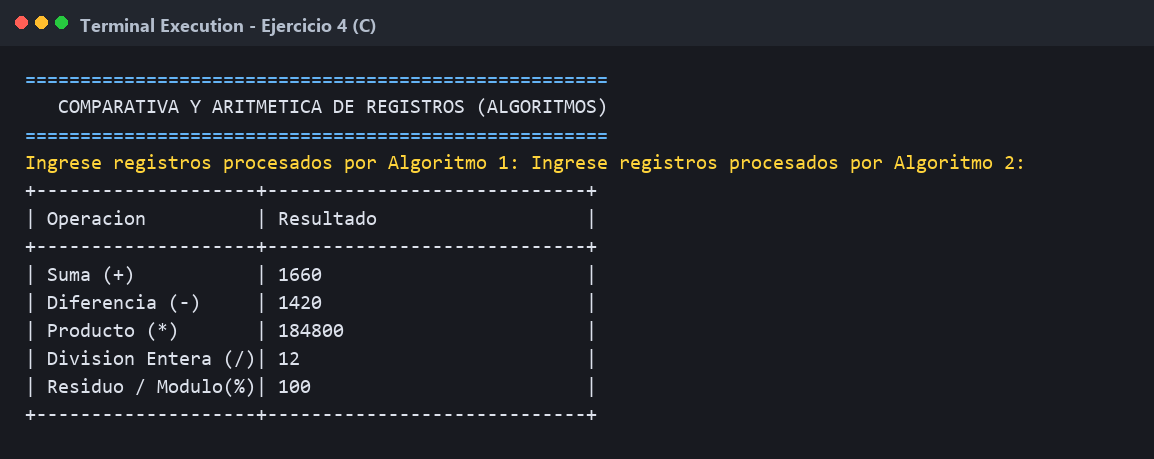
\includegraphics[width=0.92\textwidth]{captura_ejercicio4.png}
\end{center}

\vspace{5mm}
\hrule
\newpage

% ========================================================
% EJERCICIO 5
% ========================================================
\section*{Ejercicio 5: Distribución de Carga de Registros en Nodos}
\addcontentsline{toc}{section}{Ejercicio 5: Distribución de Carga de Registros en Nodos}

\noindent\textbf{Enunciado:}\\
\textit{Un conjunto de datos contiene un determinado número de registros que deben distribuirse entre varios nodos de procesamiento. Desarrolle un programa en C que solicite el número total de registros y el número de nodos, determine cuántos registros procesa cada nodo y cuántos quedan sin distribuir uniformemente.}

\subsection*{Análisis del Algoritmo}
Se aplica la propiedad del algoritmo de la división euclidiana:
\[ \text{total} = \text{nodos} \times q + r \]
Donde $q = \lfloor \text{total} / \text{nodos} \rfloor$ representa la carga asignada a cada nodo de cómputo y $r = \text{total} \pmod{\text{nodos}}$ son los registros que no pueden ser repartidos de forma estrictamente homogénea.

\subsection*{Código Fuente en C (\texttt{ejercicio5.c})}
\noindent\textbf{Enlace al Repositorio:} \url{https://github.com/henrymamani-alt/henry-ejercicios/blob/main/Tarea_1_Estructuras_Basicas/codigo/ejercicio5.c}

\begin{lstlisting}[language=C]
#include <stdio.h>

int main() {
    int total_registros;
    int num_nodos;

    printf("=====================================================\n");
    printf("    DISTRIBUCION DE CARGA ENTRE NODOS DE COMPUTO     \n");
    printf("=====================================================\n");

    printf("Ingrese el numero total de registros del dataset: ");
    scanf("%d", &total_registros);

    printf("Ingrese el numero de nodos de procesamiento: ");
    scanf("%d", &num_nodos);

    if (num_nodos <= 0 || total_registros < 0) {
        printf("Error: El numero de nodos debe ser mayor a 0 y los registros no negativos.\n");
        return 1;
    }

    int registros_por_nodo = total_registros / num_nodos;
    int registros_restantes = total_registros % num_nodos;

    printf("\n---------------- REPARTO DE CARGA DE TRABAJO --------\n");
    printf(" Total de registros recibidos      : %d\n", total_registros);
    printf(" Cantidad de nodos disponibles     : %d\n", num_nodos);
    printf(" Registros procesados por cada nodo: %d\n", registros_por_nodo);
    printf(" Registros sin distribuir uniforme : %d\n", registros_restantes);
    printf(" Verificacion (nodos*carga + resto): %d * %d + %d = %d\n",
           num_nodos, registros_por_nodo, registros_restantes,
           (num_nodos * registros_por_nodo + registros_restantes));
    printf("-----------------------------------------------------\n");

    return 0;
}
\end{lstlisting}

\subsection*{Evidencia de Ejecución}
\begin{center}
    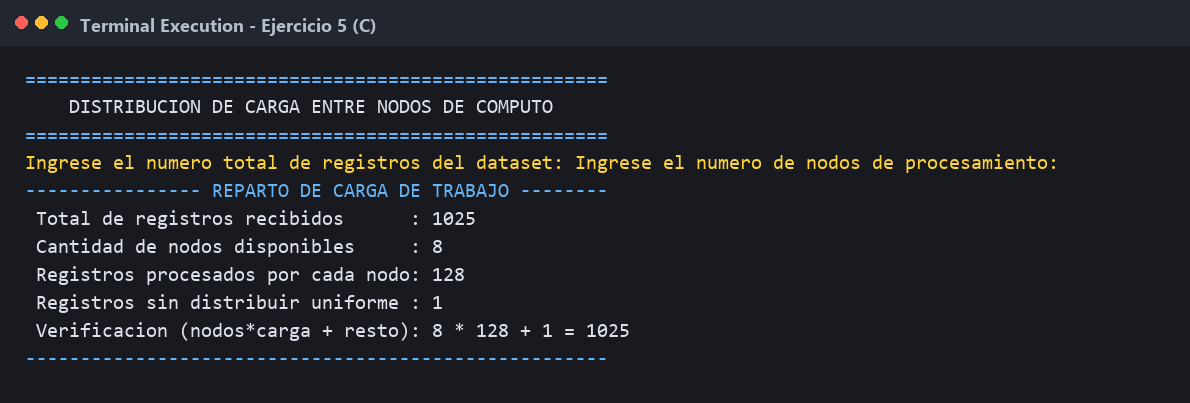
\includegraphics[width=0.92\textwidth]{captura_ejercicio5.png}
\end{center}

\vspace{5mm}
\hrule
\newpage

% ========================================================
% EJERCICIO 6
% ========================================================
\section*{Ejercicio 6: Modificación Secuencial de Variable Acumulada}
\addcontentsline{toc}{section}{Ejercicio 6: Modificación Secuencial de Variable Acumulada}

\noindent\textbf{Enunciado:}\\
\textit{Durante un proceso iterativo, una variable representa el número acumulado de registros válidos. Desarrolle un programa en C que inicialice la variable en 4, incremente su valor en 3 y posteriormente duplique el resultado. Muestre el estado de la variable después de cada operación.}

\subsection*{Análisis del Algoritmo}
Se demuestra el comportamiento temporal de una variable de estado en memoria:
\begin{enumerate}
    \item Estado Inicial: $\text{valor}_0 = 4$
    \item Asignación aditiva: $\text{valor}_1 = \text{valor}_0 + 3 = 7$ (usando operador \texttt{+=})
    \item Asignación multiplicativa: $\text{valor}_2 = \text{valor}_1 \times 2 = 14$ (usando operador \texttt{*=})
\end{enumerate}

\subsection*{Código Fuente en C (\texttt{ejercicio6.c})}
\noindent\textbf{Enlace al Repositorio:} \url{https://github.com/henrymamani-alt/henry-ejercicios/blob/main/Tarea_1_Estructuras_Basicas/codigo/ejercicio6.c}

\begin{lstlisting}[language=C]
#include <stdio.h>

int main() {
    int registros_acumulados;

    printf("=====================================================\n");
    printf("   SEGUIMIENTO DE ESTADO DE VARIABLE ACUMULADA       \n");
    printf("=====================================================\n");

    // 1. Inicializacion en 4
    registros_acumulados = 4;
    printf("[Paso 1] Inicializacion:\n");
    printf("         registros_acumulados = %d\n\n", registros_acumulados);

    // 2. Incremento en 3
    registros_acumulados += 3;
    printf("[Paso 2] Incremento en 3 (operador += 3):\n");
    printf("         registros_acumulados = %d\n\n", registros_acumulados);

    // 3. Duplicacion del resultado
    registros_acumulados *= 2;
    printf("[Paso 3] Duplicar resultado (operador *= 2):\n");
    printf("         registros_acumulados = %d\n\n", registros_acumulados);

    printf("=====================================================\n");
    printf(" Estado final del acumulador de registros: %d\n", registros_acumulados);
    printf("=====================================================\n");

    return 0;
}
\end{lstlisting}

\subsection*{Evidencia de Ejecución}
\begin{center}
    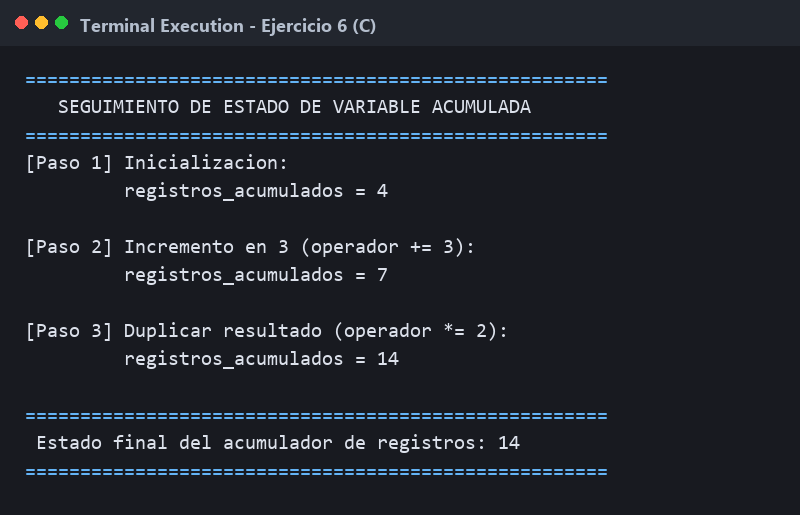
\includegraphics[width=0.92\textwidth]{captura_ejercicio6.png}
\end{center}

\vspace{5mm}
\hrule
\newpage

% ========================================================
% EJERCICIO 7
% ========================================================
\section*{Ejercicio 7: Control de Calidad y Condiciones de Dataset}
\addcontentsline{toc}{section}{Ejercicio 7: Control de Calidad y Condiciones de Dataset}

\noindent\textbf{Enunciado:}\\
\textit{Un conjunto de datos será aceptado para análisis únicamente si contiene al menos 100 observaciones válidas y presenta un porcentaje de datos completos igual o superior al 70 \%. Desarrolle un programa en C que solicite ambos valores y determine si el conjunto de datos cumple las condiciones mínimas para ser analizado.}

\subsection*{Análisis del Algoritmo}
Se evalúan simultáneamente dos restricciones cuantitativas mediante conjunción booleana:
\[ \text{Aceptado} \iff (\text{observaciones} \ge 100) \land (\text{completitud} \ge 70.0\%) \]
Si no se satisface, el programa desglosa cuál de las dos condiciones no fue cumplida.

\subsection*{Código Fuente en C (\texttt{ejercicio7.c})}
\noindent\textbf{Enlace al Repositorio:} \url{https://github.com/henrymamani-alt/henry-ejercicios/blob/main/Tarea_1_Estructuras_Basicas/codigo/ejercicio7.c}

\begin{lstlisting}[language=C]
#include <stdio.h>
#include <stdbool.h>

int main() {
    int observaciones_validas;
    double porcentaje_completos;

    printf("=====================================================\n");
    printf("     CONTROL DE CALIDAD DE CONJUNTO DE DATOS         \n");
    printf("=====================================================\n");

    printf("Ingrese la cantidad de observaciones validas: ");
    scanf("%d", &observaciones_validas);

    printf("Ingrese el porcentaje de datos completos (0 - 100 %%): ");
    scanf("%lf", &porcentaje_completos);

    // Criterios minimos: obs >= 100 y pct >= 70.0%
    bool cumple_obs = (observaciones_validas >= 100);
    bool cumple_pct = (porcentaje_completos >= 70.0);
    bool aceptado = cumple_obs && cumple_pct;

    printf("\n---------------- EVALUACION DE CRITERIOS ------------\n");
    printf(" 1. Observaciones validas (>= 100): %d [%s]\n",
           observaciones_validas, cumple_obs ? "CUMPLE" : "NO CUMPLE");
    printf(" 2. Datos completos (>= 70.00%%)   : %.2f%% [%s]\n",
           porcentaje_completos, cumple_pct ? "CUMPLE" : "NO CUMPLE");
    printf("-----------------------------------------------------\n");

    if (aceptado) {
        printf(" >> RESULTADO: CONJUNTO DE DATOS ACEPTADO PARA ANALISIS.\n");
    } else {
        printf(" >> RESULTADO: CONJUNTO DE DATOS RECHAZADO.\n");
        printf("    Motivo(s): ");
        if (!cumple_obs) printf("[Faltan observaciones minimas] ");
        if (!cumple_pct) printf("[Porcentaje de completitud insuficiente] ");
        printf("\n");
    }
    printf("-----------------------------------------------------\n");

    return 0;
}
\end{lstlisting}

\subsection*{Evidencia de Ejecución}
\begin{center}
    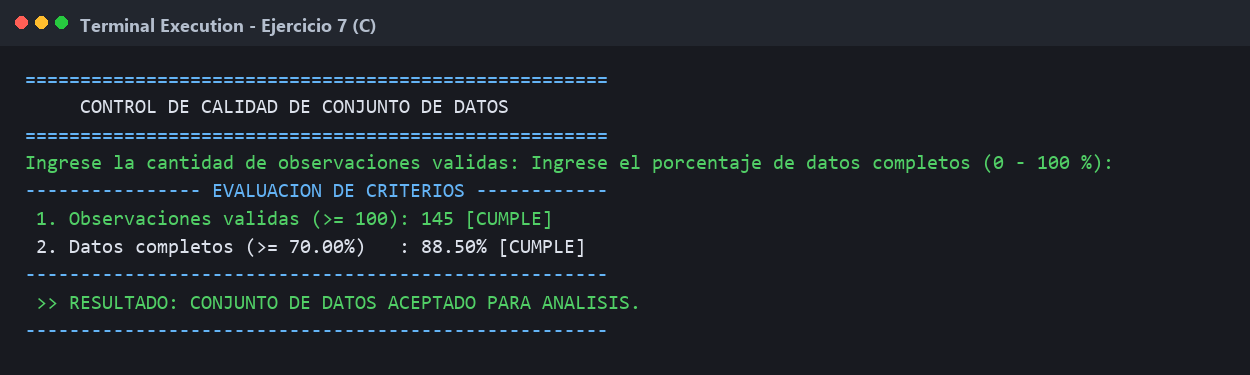
\includegraphics[width=0.92\textwidth]{captura_ejercicio7.png}
\end{center}

\vspace{5mm}
\hrule
\newpage

% ========================================================
% EJERCICIO 8
% ========================================================
\section*{Ejercicio 8: Incorporación de Observaciones con Operadores Lógicos}
\addcontentsline{toc}{section}{Ejercicio 8: Incorporación de Observaciones con Operadores Lógicos}

\noindent\textbf{Enunciado:}\\
\textit{Para incorporar una observación a un análisis, se requiere que el individuo tenga una edad mayor o igual que 18 años y que el registro haya sido validado. Desarrolle un programa en C que solicite ambos datos y utilice operadores lógicos para determinar si la observación puede incorporarse al conjunto de datos.}

\subsection*{Análisis del Algoritmo}
Se estructura una regla de admisión basada en dos condiciones deterministas:
\[ \text{Incorporar} = (\text{edad} \ge 18) \land (\text{validado} == 1) \]
La evaluación por cortocircuito del operador \texttt{\&\&} optimiza la verificación en memoria.

\subsection*{Código Fuente en C (\texttt{ejercicio8.c})}
\noindent\textbf{Enlace al Repositorio:} \url{https://github.com/henrymamani-alt/henry-ejercicios/blob/main/Tarea_1_Estructuras_Basicas/codigo/ejercicio8.c}

\begin{lstlisting}[language=C]
#include <stdio.h>
#include <stdbool.h>

int main() {
    int edad;
    int estado_validacion; // 1 = Validado, 0 = No validado

    printf("=====================================================\n");
    printf("   FILTRO DE ADMISION DE OBSERVACIONES AL ESTUDIO    \n");
    printf("=====================================================\n");

    printf("Ingrese la edad del individuo: ");
    scanf("%d", &edad);

    printf("Ha sido validado el registro? (1 = Si / 0 = No): ");
    scanf("%d", &estado_validacion);

    bool es_mayor_edad = (edad >= 18);
    bool esta_validado = (estado_validacion == 1);

    // Operador logico AND (&&)
    bool puede_incorporarse = es_mayor_edad && esta_validado;

    printf("\n---------------- VERIFICACION DE CONDICIONES ---------\n");
    printf(" Condicion 1 (Edad >= 18)   : %d anios -> %s\n", edad, es_mayor_edad ? "VERDADERO" : "FALSO");
    printf(" Condicion 2 (Validado == 1): %d -> %s\n", estado_validacion, esta_validado ? "VERDADERO" : "FALSO");
    printf(" Expresion logica           : (edad >= 18) && (validado == 1)\n");
    printf(" Evaluacion                 : %s\n", puede_incorporarse ? "TRUE" : "FALSE");
    printf("-----------------------------------------------------\n");

    if (puede_incorporarse) {
        printf(" >> DICTAMEN: La observacion PUEDE incorporarse al conjunto de datos.\n");
    } else {
        printf(" >> DICTAMEN: La observacion NO PUEDE incorporarse al analisis.\n");
    }
    printf("=====================================================\n");

    return 0;
}
\end{lstlisting}

\subsection*{Evidencia de Ejecución}
\begin{center}
    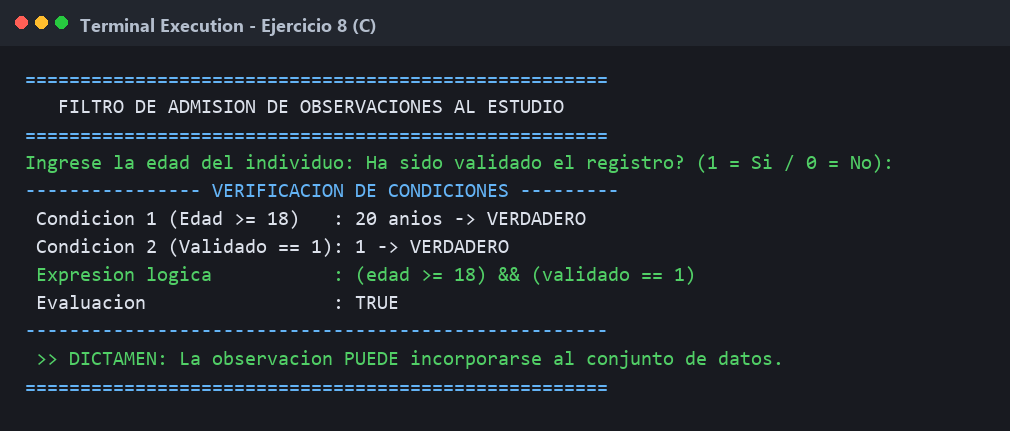
\includegraphics[width=0.92\textwidth]{captura_ejercicio8.png}
\end{center}

\vspace{5mm}
\hrule
\newpage

% ========================================================
% EJERCICIO 9
% ========================================================
\section*{Ejercicio 9: Clasificación Climática de Temperatura por Sensor}
\addcontentsline{toc}{section}{Ejercicio 9: Clasificación Climática de Temperatura por Sensor}

\noindent\textbf{Enunciado:}\\
\textit{Un sensor registra temperaturas ambientales utilizadas posteriormente en un análisis climático. Desarrolle un programa en C que solicite una temperatura y la clasifique como Congelación si es menor que 0 °C, Frío si está entre 0 y 20 °C, y Templado si supera los 20 °C.}

\subsection*{Análisis del Algoritmo}
Se implementa una estructura selectiva múltiple:
\begin{itemize}
    \item $T < 0 \, ^\circ\text{C} \implies \textbf{Congelación}$
    \item $0 \le T \le 20 \, ^\circ\text{C} \implies \textbf{Frío}$
    \item $T > 20 \, ^\circ\text{C} \implies \textbf{Templado}$
\end{itemize}

\subsection*{Código Fuente en C (\texttt{ejercicio9.c})}
\noindent\textbf{Enlace al Repositorio:} \url{https://github.com/henrymamani-alt/henry-ejercicios/blob/main/Tarea_1_Estructuras_Basicas/codigo/ejercicio9.c}

\begin{lstlisting}[language=C]
#include <stdio.h>

int main() {
    float temperatura;

    printf("=====================================================\n");
    printf("      CLASIFICACION DE TEMPERATURAS CLIMATICAS       \n");
    printf("=====================================================\n");

    printf("Ingrese la temperatura registrada por el sensor (en C): ");
    if (scanf("%f", &temperatura) != 1) {
        printf("Error: Registro de temperatura invalido.\n");
        return 1;
    }

    printf("\n---------------- RESULTADO DE EVALUACION -------------\n");
    printf(" Temperatura sensada: %.2f C\n", temperatura);
    printf(" Clasificacion      : ");

    if (temperatura < 0.0f) {
        printf("CONGELACION (< 0 C)\n");
        printf(" Observacion        : Condiciones bajo el punto de congelacion.\n");
    } else if (temperatura >= 0.0f && temperatura <= 20.0f) {
        printf("FRIO (0 C a 20 C)\n");
        printf(" Observacion        : Rango termico bajo, caracteristico de zonas andinas.\n");
    } else {
        printf("TEMPLADO (> 20 C)\n");
        printf(" Observacion        : Rango termico moderado y calido.\n");
    }
    printf("-----------------------------------------------------\n");

    return 0;
}
\end{lstlisting}

\subsection*{Evidencia de Ejecución}
\begin{center}
    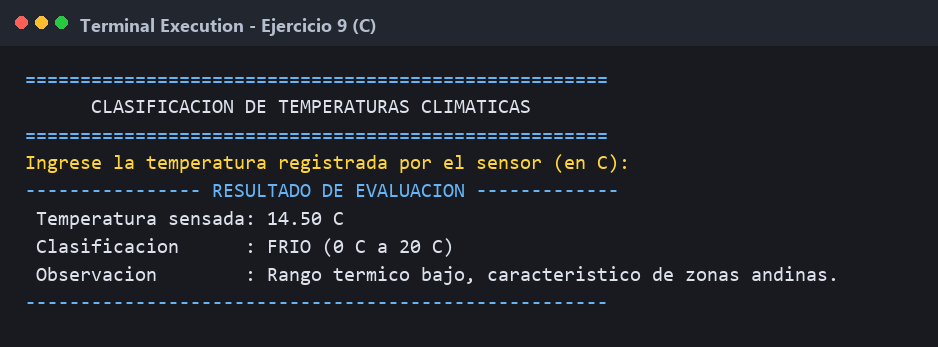
\includegraphics[width=0.92\textwidth]{captura_ejercicio9.png}
\end{center}

\vspace{5mm}
\hrule
\newpage

% ========================================================
% EJERCICIO 10
% ========================================================
\section*{Ejercicio 10: Ciclo \texttt{for}, Media y Observaciones Superiores (C++)}
\addcontentsline{toc}{section}{Ejercicio 10: Ciclo for, Media y Observaciones Superiores (C++)}

\noindent\textbf{Enunciado:}\\
\textit{Un investigador dispone de las mediciones de una variable para 10 observaciones. Desarrolle un programa en C++ que utilice un ciclo for para ingresar los valores, calcule la media aritmética y determine cuántas observaciones se encuentran por encima de dicha media.}

\subsection*{Análisis del Algoritmo}
En C++, se utiliza el flujo de entrada \texttt{cin} y salida \texttt{cout}. Un bucle \texttt{for} recopila los 10 registros y acumula la sumatoria. Se computa $\bar{x} = \frac{\sum x_i}{10}$ y un segundo recorrido identifica las observaciones que satisfacen $x_i > \bar{x}$.

\subsection*{Código Fuente en C++ (\texttt{ejercicio10.cpp})}
\noindent\textbf{Enlace al Repositorio:} \url{https://github.com/henrymamani-alt/henry-ejercicios/blob/main/Tarea_1_Estructuras_Basicas/codigo/ejercicio10.cpp}

\begin{lstlisting}[language=C++]
#include <iostream>
#include <iomanip>

using namespace std;

int main() {
    const int N = 10;
    double mediciones[N];
    double suma = 0.0;
    double media = 0.0;
    int conteo_superiores = 0;

    cout << "=====================================================" << endl;
    cout << "  ANALISIS ESTADISTICO DE 10 MEDICIONES (C++)        " << endl;
    cout << "=====================================================" << endl;

    // Ciclo for para ingresar los valores
    for (int i = 0; i < N; i++) {
        cout << "Ingrese la medicion [" << (i + 1) << "/" << N << "]: ";
        cin >> mediciones[i];
        suma += mediciones[i];
    }

    // Calculo de la media aritmetica
    media = suma / N;

    // Determinar cuantas observaciones estan por encima de la media
    for (int i = 0; i < N; i++) {
        if (mediciones[i] > media) {
            conteo_superiores++;
        }
    }

    cout << fixed << setprecision(2);
    cout << "\n---------------- RESUMEN ESTADISTICO ----------------" << endl;
    cout << " Suma total acumulada            : " << suma << endl;
    cout << " Media aritmetica del grupo      : " << media << endl;
    cout << " Observaciones mayores a la media: " << conteo_superiores << " de " << N << endl;
    cout << "\nDetalle de observaciones y clasificacion respecto a la media:" << endl;
    for (int i = 0; i < N; i++) {
        cout << " Obs " << setw(2) << (i + 1) << ": " << setw(7) << mediciones[i];
        if (mediciones[i] > media) {
            cout << "  -> Por encima de la media (+)" << endl;
        } else if (mediciones[i] < media) {
            cout << "  -> Por debajo de la media (-)" << endl;
        } else {
            cout << "  -> Igual a la media" << endl;
        }
    }
    cout << "-----------------------------------------------------" << endl;

    return 0;
}
\end{lstlisting}

\subsection*{Evidencia de Ejecución}
\begin{center}
    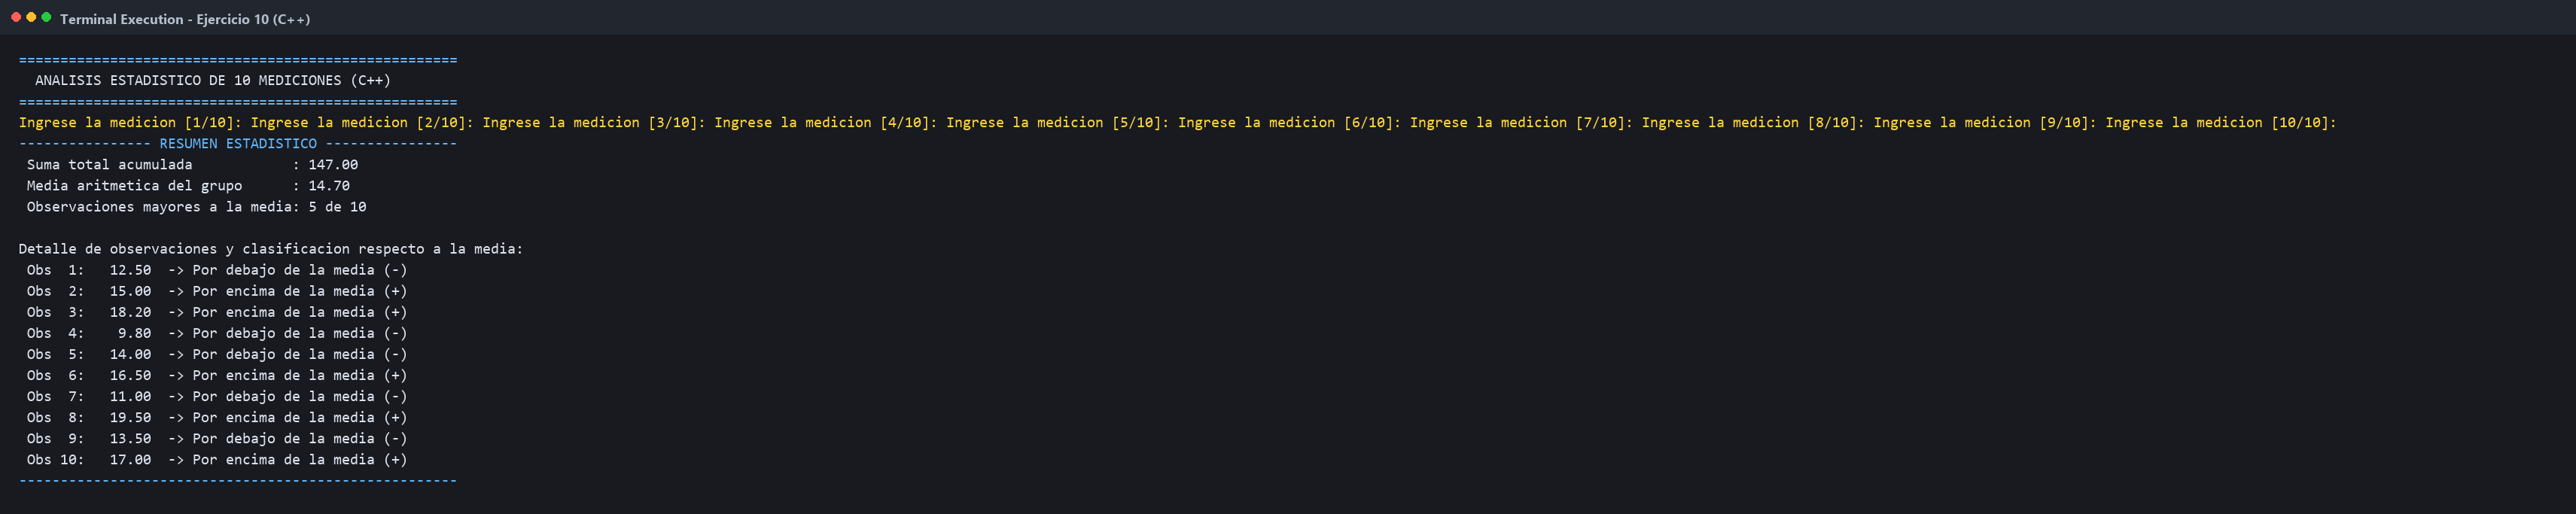
\includegraphics[width=0.92\textwidth]{captura_ejercicio10.png}
\end{center}

\vspace{5mm}
\hrule
\newpage

% ========================================================
% EJERCICIO 11
% ========================================================
\section*{Ejercicio 11: Control de Autenticación con Ciclo \texttt{while} (C++)}
\addcontentsline{toc}{section}{Ejercicio 11: Control de Autenticación con Ciclo while (C++)}

\noindent\textbf{Enunciado:}\\
\textit{Durante la carga manual de datos, el sistema requiere una clave numérica de acceso. Desarrolle un programa en C ++ que solicite repetidamente la contraseña mediante un ciclo while, contabilice el número de intentos realizados y finalice cuando se ingrese la clave correcta.}

\subsection*{Análisis del Algoritmo}
Se emplea un ciclo condicional indeterminado \texttt{while(!acceso\_concedido)}. Se incrementa el contador de intentos en cada ciclo. Al ingresar la clave correcta (\texttt{2026}), la bandera cambia de estado y el bucle termina informando el balance de intentos.

\subsection*{Código Fuente en C++ (\texttt{ejercicio11.cpp})}
\noindent\textbf{Enlace al Repositorio:} \url{https://github.com/henrymamani-alt/henry-ejercicios/blob/main/Tarea_1_Estructuras_Basicas/codigo/ejercicio11.cpp}

\begin{lstlisting}[language=C++]
#include <iostream>

using namespace std;

int main() {
    const int CLAVE_CORRECTA = 2026;
    int clave_ingresada = 0;
    int intentos = 0;
    bool acceso_concedido = false;

    cout << "=====================================================" << endl;
    cout << "  SISTEMA DE AUTENTICACION PARA CARGA DE DATOS (C++) " << endl;
    cout << "=====================================================" << endl;
    cout << "(Clave de acceso predefinida: 2026)" << endl << endl;

    // Ciclo while para solicitar repetidamente la clave
    while (!acceso_concedido) {
        intentos++;
        cout << "Intento #" << intentos << " - Ingrese la clave numerica de acceso: ";
        cin >> clave_ingresada;

        if (clave_ingresada == CLAVE_CORRECTA) {
            acceso_concedido = true;
            cout << "\n[!] ACCESO CONCEDIDO." << endl;
            cout << "    Bienvenido al modulo de carga de datos." << endl;
        } else {
            cout << "[-] Clave incorrecta. Acceso denegado. Intente nuevamente.\n" << endl;
        }
    }

    cout << "-----------------------------------------------------" << endl;
    cout << " Resumen de inicio de sesion:" << endl;
    cout << " Numero total de intentos realizados: " << intentos << endl;
    cout << " Estado final: Autenticacion exitosa." << endl;
    cout << "=====================================================" << endl;

    return 0;
}
\end{lstlisting}

\subsection*{Evidencia de Ejecución}
\begin{center}
    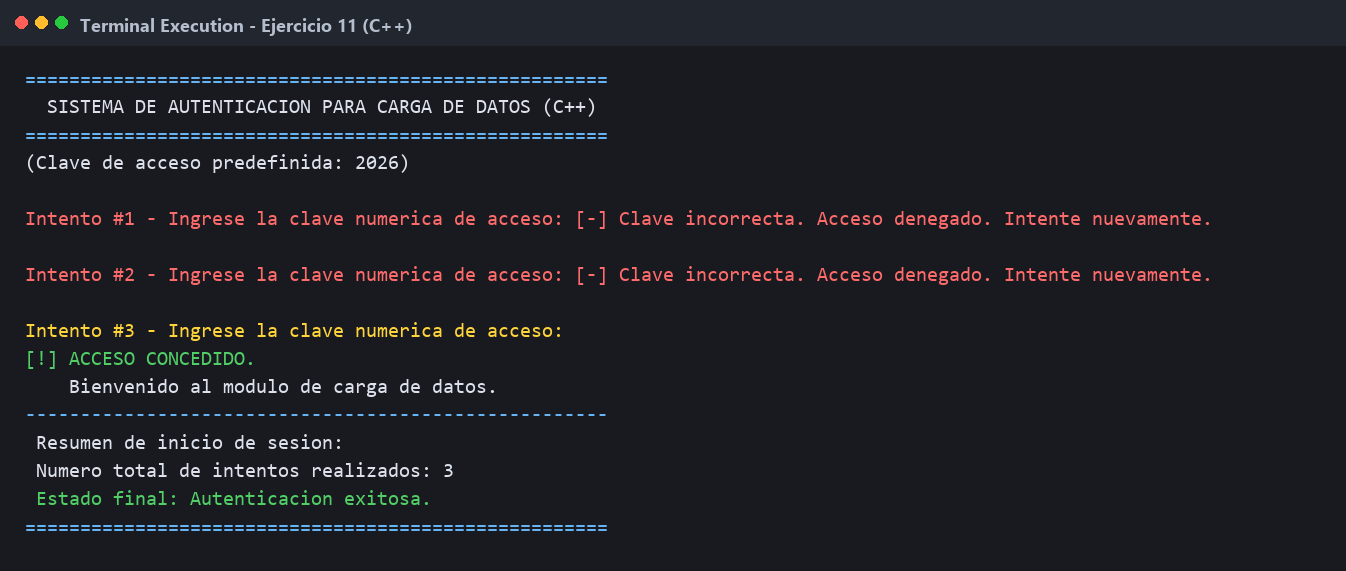
\includegraphics[width=0.92\textwidth]{captura_ejercicio11.png}
\end{center}

\vspace{5mm}
\hrule
\newpage

% ========================================================
% EJERCICIO 12
% ========================================================
\section*{Ejercicio 12: Control de Secuencias con \texttt{continue} y \texttt{break} (C++)}
\addcontentsline{toc}{section}{Ejercicio 12: Control de Secuencias con continue y break (C++)}

\noindent\textbf{Enunciado:}\\
\textit{Desarrolle un programa en C++ que procese una secuencia de 10 mediciones. Los valores negativos deben considerarse inválidos y omitirse mediante continue. Si se introduce el valor 999, el procesamiento debe finalizar mediante break. Al terminar, muestre cuántos valores válidos fueron procesados.}

\subsection*{Análisis del Algoritmo}
Este ejercicio ilustra la manipulación explícita del flujo de ejecución:
\begin{itemize}
    \item \texttt{continue}: Omite la contabilización de datos anómalos (valores negativos).
    \item \texttt{break}: Interrumpe de manera inmediata el procesamiento ante la presencia del valor centinela \texttt{999}.
\end{itemize}

\subsection*{Código Fuente en C++ (\texttt{ejercicio12.cpp})}
\noindent\textbf{Enlace al Repositorio:} \url{https://github.com/henrymamani-alt/henry-ejercicios/blob/main/Tarea_1_Estructuras_Basicas/codigo/ejercicio12.cpp}

\begin{lstlisting}[language=C++]
#include <iostream>
#include <vector>

using namespace std;

int main() {
    const int MAX_MEDICIONES = 10;
    int validos = 0;
    double valor;
    vector<double> lista_validos;

    cout << "=====================================================" << endl;
    cout << "  PROCESAMIENTO DE MEDICIONES CON CONTINUE Y BREAK   " << endl;
    cout << "=====================================================" << endl;
    cout << "Instrucciones: Se esperan hasta 10 mediciones.\n"
         << "- Valores negativos: Se omiten con continue.\n"
         << "- Valor 999        : Finaliza la captura con break.\n" << endl;

    for (int i = 1; i <= MAX_MEDICIONES; i++) {
        cout << "Entrada " << i << " de " << MAX_MEDICIONES << " - Ingrese medicion: ";
        cin >> valor;

        // Finalizacion inmediata si se introduce 999 mediante break
        if (valor == 999) {
            cout << ">> [BREAK] Se introdujo el codigo de parada 999. Finalizando proceso..." << endl;
            break;
        }

        // Omitir valores negativos mediante continue
        if (valor < 0) {
            cout << ">> [CONTINUE] Medicion negativa (" << valor << ") invalida. Se omite." << endl;
            continue;
        }

        // Si es valido, se contabiliza y almacena
        validos++;
        lista_validos.push_back(valor);
        cout << "   -> Medicion " << valor << " registrada correctamente como valida." << endl;
    }

    cout << "\n---------------- RESUMEN FINAL DEL PROCESAMIENTO ----" << endl;
    cout << " Total de valores validos procesados: " << validos << endl;
    cout << " Valores validos registrados: ";
    if (validos == 0) {
        cout << "Ninguno";
    } else {
        for (size_t j = 0; j < lista_validos.size(); j++) {
            cout << lista_validos[j] << (j + 1 < lista_validos.size() ? ", " : "");
        }
    }
    cout << "\n-----------------------------------------------------" << endl;

    return 0;
}
\end{lstlisting}

\subsection*{Evidencia de Ejecución}
\begin{center}
    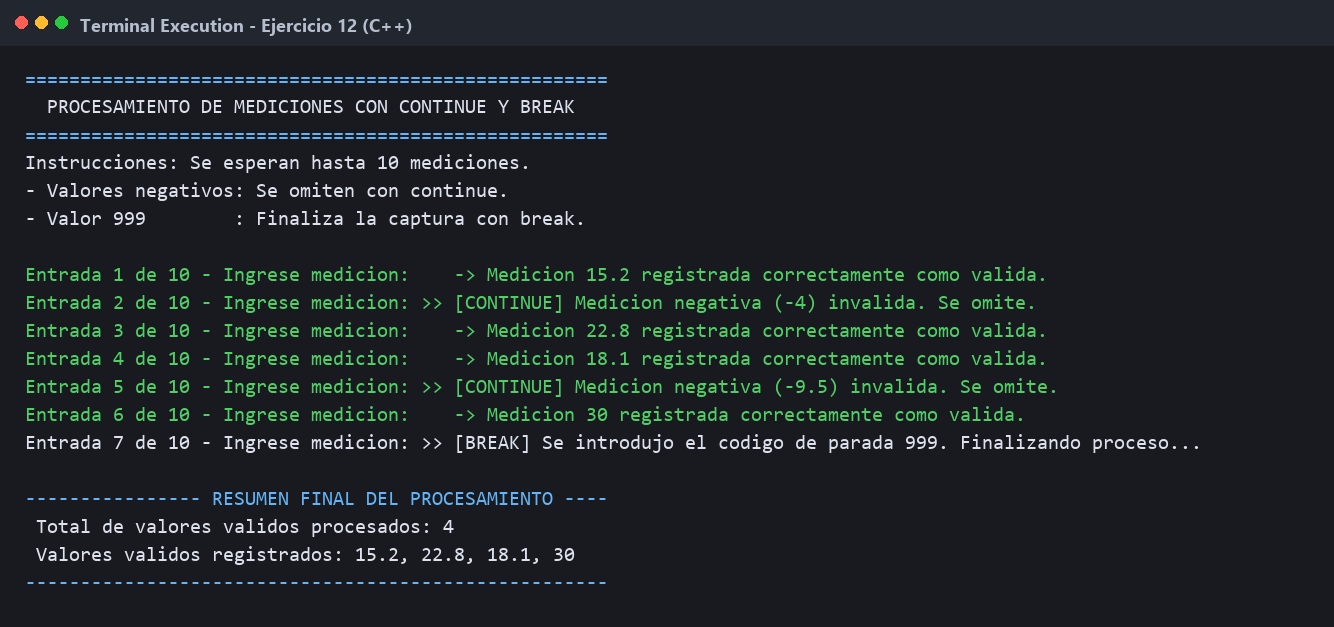
\includegraphics[width=0.92\textwidth]{captura_ejercicio12.png}
\end{center}

\vspace{5mm}
\hrule
\newpage

% ========================================================
% EJERCICIO 13
% ========================================================
\section*{Ejercicio 13: Arreglos y Métricas Estadísticas de Edades}
\addcontentsline{toc}{section}{Ejercicio 13: Arreglos y Métricas Estadísticas de Edades}

\noindent\textbf{Enunciado:}\\
\textit{Un conjunto de datos contiene las edades de 10 participantes de un estudio. Desarrolle un programa en C que almacene los valores en un arreglo y determine la edad mínima, edad máxima, media y número de participantes cuya edad supera la media del grupo.}

\subsection*{Análisis del Algoritmo}
Se emplea un arreglo estático \texttt{int edades[10]}. Se procesan en una sola pasada inicial el cálculo de la sumatoria y la identificación de valores extremos:
\[ \min = \min_{i} \{x_i\}, \quad \max = \max_{i} \{x_i\} \]
Posteriormente, con la media $\bar{x} = \frac{\sum x_i}{10}$, se filtran aquellos participantes que superan dicho umbral.

\subsection*{Código Fuente en C (\texttt{ejercicio13.c})}
\noindent\textbf{Enlace al Repositorio:} \url{https://github.com/henrymamani-alt/henry-ejercicios/blob/main/Tarea_1_Estructuras_Basicas/codigo/ejercicio13.c}

\begin{lstlisting}[language=C]
#include <stdio.h>

#define N 10

int main() {
    int edades[N];
    int min_edad, max_edad;
    double suma = 0.0, media = 0.0;
    int sobre_media = 0;

    printf("=====================================================\n");
    printf("   ESTUDIO DEMOGRAFICO: ANALISIS DE 10 EDADES        \n");
    printf("=====================================================\n");

    for (int i = 0; i < N; i++) {
        printf("Ingrese la edad del participante [%d/%d]: ", i + 1, N);
        scanf("%d", &edades[i]);
        suma += edades[i];
    }

    // Inicializar min y max con el primer elemento
    min_edad = edades[0];
    max_edad = edades[0];

    for (int i = 1; i < N; i++) {
        if (edades[i] < min_edad) min_edad = edades[i];
        if (edades[i] > max_edad) max_edad = edades[i];
    }

    media = suma / N;

    for (int i = 0; i < N; i++) {
        if (edades[i] > media) {
            sobre_media++;
        }
    }

    printf("\n---------------- RESULTADOS ESTADISTICOS ------------\n");
    printf(" Lista de edades ingresadas: ");
    for (int i = 0; i < N; i++) {
        printf("%d%s", edades[i], (i < N - 1) ? ", " : "\n");
    }
    printf(" Edad minima en el grupo    : %d anios\n", min_edad);
    printf(" Edad maxima en el grupo    : %d anios\n", max_edad);
    printf(" Edad media del grupo       : %.2f anios\n", media);
    printf(" Participantes con edad > media: %d participantes\n", sobre_media);
    printf("-----------------------------------------------------\n");

    return 0;
}
\end{lstlisting}

\subsection*{Evidencia de Ejecución}
\begin{center}
    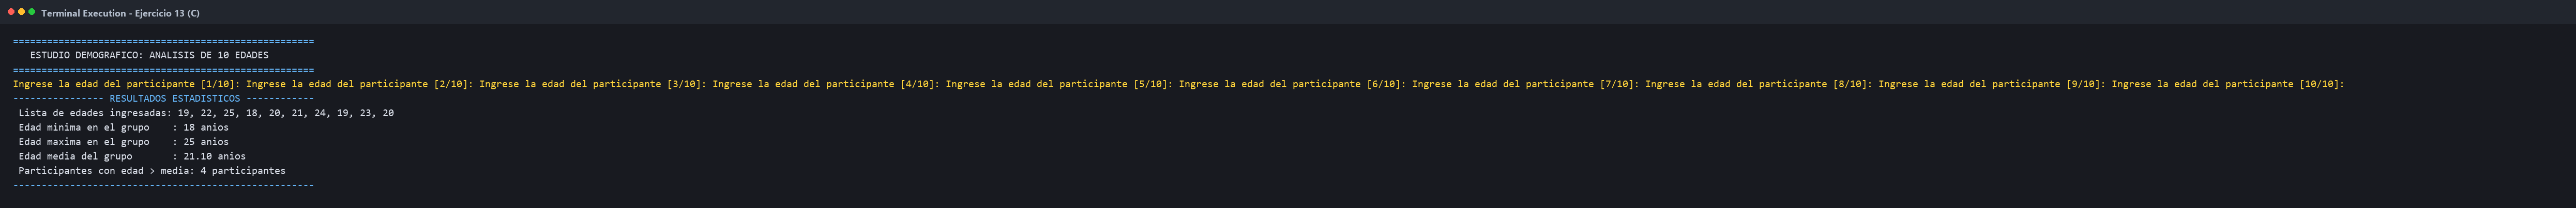
\includegraphics[width=0.92\textwidth]{captura_ejercicio13.png}
\end{center}

\vspace{5mm}
\hrule
\newpage

% ========================================================
% EJERCICIO 14
% ========================================================
\section*{Ejercicio 14: Comparación Empírica de Complejidad $O(n)$ vs $O(n^2)$}
\addcontentsline{toc}{section}{Ejercicio 14: Comparación Empírica de Complejidad O(n) vs O(n2)}

\noindent\textbf{Enunciado:}\\
\textit{Desarrolle un programa en C que permita ingresar un valor n y compare dos procedimientos: el primero debe realizar un solo recorrido de n elementos y el segundo debe utilizar dos ciclos anidados de n iteraciones. Utilice contadores para estimar el número de operaciones realizadas y relacione los resultados con complejidades aproximadas O(n) y O(n²).}

\subsection*{Análisis del Algoritmo}
Se contrastan experimentalmente las dos clases de complejidad:
\begin{itemize}
    \item Recorrido simple: Realiza exactamente $n$ operaciones elementales ($\mathcal{O}(n)$).
    \item Doble ciclo anidado: Ejecuta $\sum_{i=1}^n \sum_{j=1}^n 1 = n \times n = n^2$ operaciones ($\mathcal{O}(n^2)$).
\end{itemize}
El factor de crecimiento relativo es precisamente $\frac{n^2}{n} = n$, corroborando el costo de las soluciones no lineales en el procesamiento de datos masivos.

\subsection*{Código Fuente en C (\texttt{ejercicio14.c})}
\noindent\textbf{Enlace al Repositorio:} \url{https://github.com/henrymamani-alt/henry-ejercicios/blob/main/Tarea_1_Estructuras_Basicas/codigo/ejercicio14.c}

\begin{lstlisting}[language=C]
#include <stdio.h>

int main() {
    int n;
    long long contador_lineal = 0;
    long long contador_cuadratico = 0;

    printf("=====================================================\n");
    printf("    ANALISIS DE COMPLEJIDAD: O(n) vs O(n^2)          \n");
    printf("=====================================================\n");

    printf("Ingrese la cantidad de elementos n (ej. 10, 50, 100, 500): ");
    if (scanf("%d", &n) != 1 || n <= 0) {
        printf("Error: Ingrese un valor entero positivo para n.\n");
        return 1;
    }

    // Procedimiento 1: Un solo recorrido de n elementos -> O(n)
    for (int i = 0; i < n; i++) {
        contador_lineal++;
    }

    // Procedimiento 2: Dos ciclos anidados de n iteraciones -> O(n^2)
    for (int i = 0; i < n; i++) {
        for (int j = 0; j < n; j++) {
            contador_cuadratico++;
        }
    }

    double ratio = (contador_lineal > 0) ? ((double)contador_cuadratico / (double)contador_lineal) : 0.0;

    printf("\n+------------------------------+--------------------+\n");
    printf("| Parametro / Procedimiento    | Valor              |\n");
    printf("+------------------------------+--------------------+\n");
    printf("| Tamanio de entrada (n)       | %-18d |\n", n);
    printf("| Operaciones Lineales O(n)    | %-18lld |\n", contador_lineal);
    printf("| Operaciones Cuadraticas O(n2)| %-18lld |\n", contador_cuadratico);
    printf("| Factor de escala (O(n2)/O(n))| %-18.2f |\n", ratio);
    printf("+------------------------------+--------------------+\n");

    printf("\nInterpretacion Teorico-Practica:\n");
    printf("1. En O(n), el crecimiento del tiempo es lineal: se realizaron exactamente n = %d ops.\n", n);
    printf("2. En O(n^2), el crecimiento es cuadratico: se realizaron exactamente n^2 = %lld ops.\n", contador_cuadratico);
    printf("3. Notese que el factor de escala es exactamente n = %.0f, lo que demuestra que al duplicar n,\n", ratio);
    printf("   el procedimiento O(n^2) incrementa su costo computacional en un factor cuadratico (x4).\n");
    printf("=====================================================\n");

    return 0;
}
\end{lstlisting}

\subsection*{Evidencia de Ejecución}
\begin{center}
    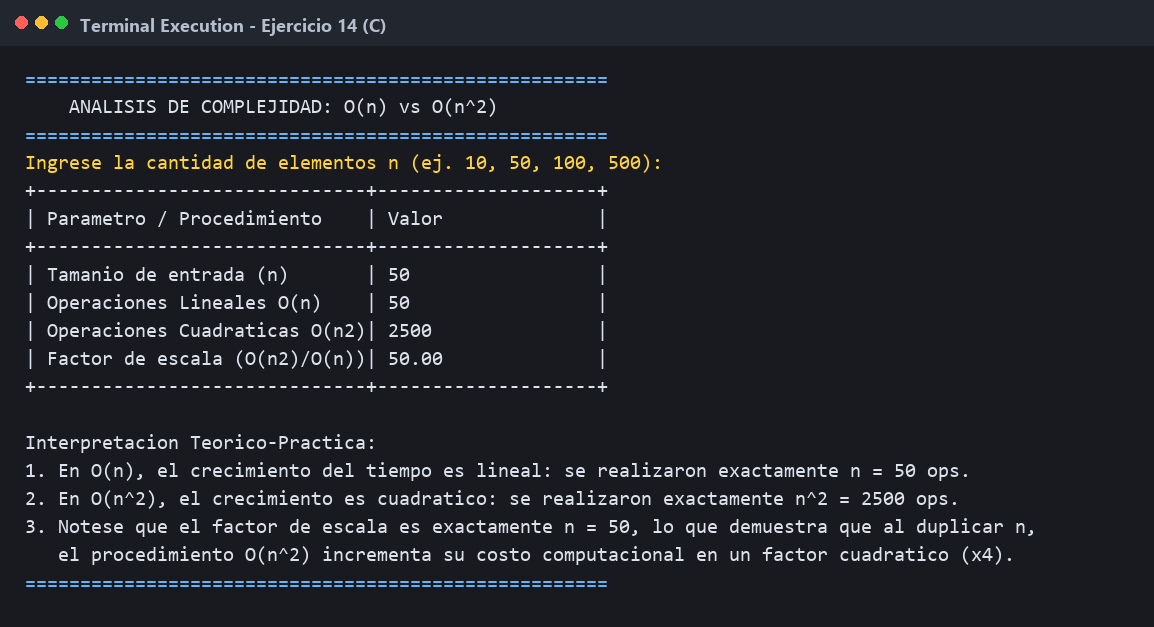
\includegraphics[width=0.92\textwidth]{captura_ejercicio14.png}
\end{center}

\vspace{5mm}
\hrule
\newpage

% ========================================================
% EJERCICIO 15
% ========================================================
\section*{Ejercicio 15: Modularidad y Funciones Estadísticas}
\addcontentsline{toc}{section}{Ejercicio 15: Modularidad y Funciones Estadísticas}

\noindent\textbf{Enunciado:}\\
\textit{Un pequeño conjunto de datos contiene tres mediciones obtenidas de una misma variable. Desarrolle un programa en C que implemente una función calcular\_promedio para recibir las tres mediciones, calcular su media y retornar el resultado. Además, implemente una segunda función que determine cuántas de las mediciones se encuentran por encima del promedio.}

\subsection*{Análisis del Algoritmo}
Se aplican los principios de programación estructurada y modularización:
\begin{enumerate}
    \item \texttt{double calcular\_promedio(double m1, double m2, double m3)}: Recibe por valor las tres muestras, realiza la media aritmética y retorna el resultado.
    \item \texttt{int contar\_superiores\_promedio(double m1, double m2, double m3, double prom)}: Evalúa cada parámetro frente al umbral promedio y retorna la cardinalidad de mediciones superiores.
\end{enumerate}

\subsection*{Código Fuente en C (\texttt{ejercicio15.c})}
\noindent\textbf{Enlace al Repositorio:} \url{https://github.com/henrymamani-alt/henry-ejercicios/blob/main/Tarea_1_Estructuras_Basicas/codigo/ejercicio15.c}

\begin{lstlisting}[language=C]
#include <stdio.h>

// Funcion 1: Recibe 3 mediciones y calcula su media aritmetica
double calcular_promedio(double m1, double m2, double m3) {
    return (m1 + m2 + m3) / 3.0;
}

// Funcion 2: Determina cuantas mediciones estan por encima del promedio
int contar_superiores_promedio(double m1, double m2, double m3, double promedio) {
    int contador = 0;
    if (m1 > promedio) contador++;
    if (m2 > promedio) contador++;
    if (m3 > promedio) contador++;
    return contador;
}

int main() {
    double m1, m2, m3;

    printf("=====================================================\n");
    printf("   MODULARIDAD: PROMEDIO Y COMPARACION DE 3 MUESTRAS \n");
    printf("=====================================================\n");

    printf("Ingrese la medicion 1: ");
    scanf("%lf", &m1);

    printf("Ingrese la medicion 2: ");
    scanf("%lf", &m2);

    printf("Ingrese la medicion 3: ");
    scanf("%lf", &m3);

    // Invocacion de la funcion calcular_promedio
    double promedio = calcular_promedio(m1, m2, m3);

    // Invocacion de la funcion contar_superiores_promedio
    int mayores = contar_superiores_promedio(m1, m2, m3, promedio);

    printf("\n---------------- RESUMEN DE RESULTADOS --------------\n");
    printf(" Mediciones ingresadas : [%.2f, %.2f, %.2f]\n", m1, m2, m3);
    printf(" Promedio calculado    : %.4f\n", promedio);
    printf(" Mediciones > promedio : %d de 3\n", mayores);

    printf("\nDetalle individual:\n");
    printf(" - Medicion 1 (%.2f): %s\n", m1, (m1 > promedio) ? "SUPERIOR al promedio" : "Menor o igual al promedio");
    printf(" - Medicion 2 (%.2f): %s\n", m2, (m2 > promedio) ? "SUPERIOR al promedio" : "Menor o igual al promedio");
    printf(" - Medicion 3 (%.2f): %s\n", m3, (m3 > promedio) ? "SUPERIOR al promedio" : "Menor o igual al promedio");
    printf("-----------------------------------------------------\n");

    return 0;
}
\end{lstlisting}

\subsection*{Evidencia de Ejecución}
\begin{center}
    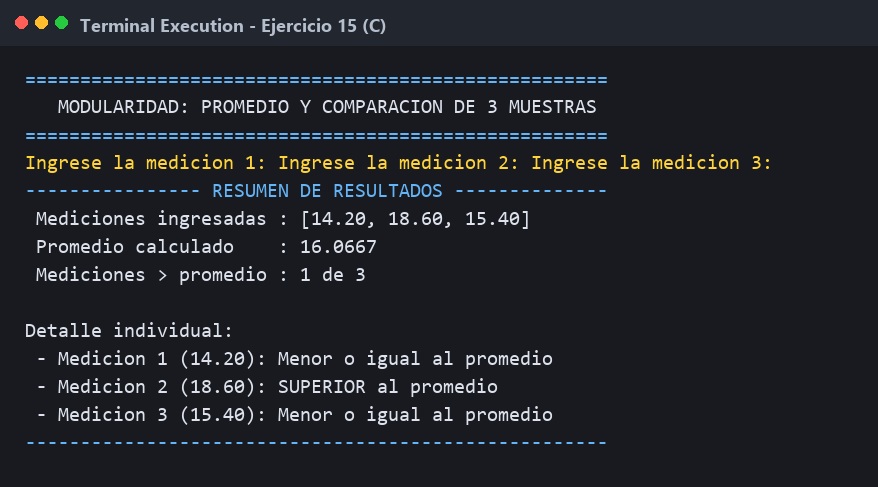
\includegraphics[width=0.92\textwidth]{captura_ejercicio15.png}
\end{center}

\vspace{5mm}
\hrule
\newpage

% ========================================================
% CONCLUSIONES
% ========================================================
\section*{Conclusiones Generales}
\addcontentsline{toc}{section}{Conclusiones Generales}

\begin{enumerate}
    \item La correcta asignación de tipos primitivos (\texttt{int}, \texttt{float}, \texttt{double}, \texttt{char}, \texttt{bool}) es un pilar básico en el diseño de algoritmos estadísticos eficientes, permitiendo un uso balanceado de memoria y evitando la pérdida innecesaria de precisión.
    \item El análisis de complejidades computacionales mediante contadores empíricos evidenció el crecimiento exponencial relativo entre algoritmos de orden $\mathcal{O}(n)$ y $\mathcal{O}(n^2)$, justificando la necesidad de optimizar bucles anidados en conjuntos de datos de gran escala.
    \item Las directivas de salto condicional (\texttt{continue} y \texttt{break}) y los ciclos de control (\texttt{while}, \texttt{for}) otorgan gran flexibilidad para el filtrado, validación y parada de procesos de ingesta de información.
    \item La modularización mediante funciones especializadas en C/C++ simplifica la depuración, permite la reutilización de código y promueve una estructura organizada acorde a los estándares de desarrollo de software profesional.
\end{enumerate}

\end{document}
